\documentclass[11pt]{beamer}
\usepackage[english]{babel}
\usetheme{Madrid}
\usecolortheme{default}

\title{\textit{THREE CURVES}}
\subtitle{20411847}
\author{He SUN}
\institute{UNNC}
\date{\today}


\begin{document}

\begin{frame}
\titlepage % makes the opening slide
\end{frame}

\begin{frame}\frametitle{TABLE OF CONTENT}
\tableofcontents
\end{frame}

\section{THREE FUNCTIONS}
\begin{frame}\frametitle{THREE FUNCTIONS}
\begin{columns}
\column{0.5\textwidth}
\begin{eqnarray*} 
\begin{cases}
y =  e^{x^3-1}\\
z =  2x\*e^{x^3-1}\\
w =  x\*\sin(x)-1
\end{cases}
\end{eqnarray*}
\column{0.5\textwidth}
\begin{figure}
\centering
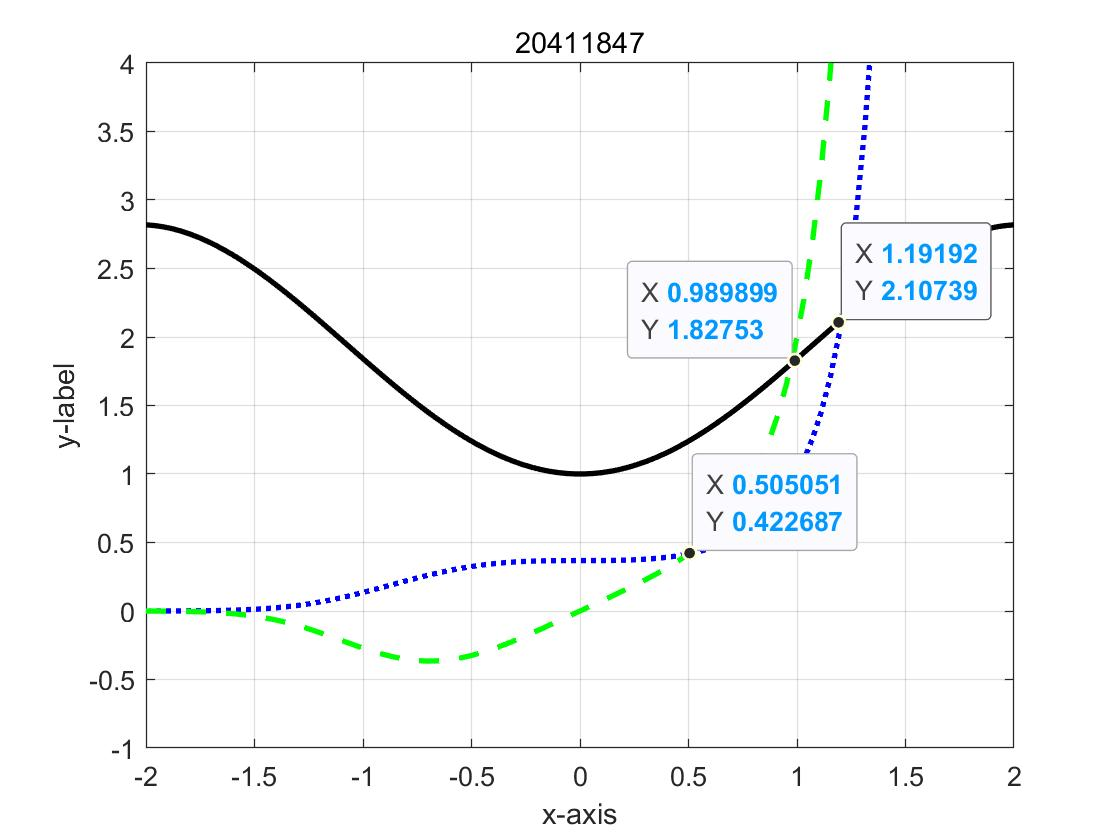
\includegraphics[width=1\textwidth]{threecurves}
\caption{\textbf{THREE CURVES}}
\end{figure}
\end{columns}
\end{frame}

\section{OBSERVATIONS}
\begin{frame}\frametitle{OBSERVATIONS}

\begin{table}[h]
\centering
\begin{tabular}{c|c|c|c}
Function&Intersection with $f$&Intersection with $g$&Intersection with $h$\\
\hline
\hline
$f(x)$&$-$&$(0.51,0.42)$&$(1.19,2.11)$\\
\hline
$g(x)$&$(0.51,0.42)$&$-$&$(0.99,1.83)$\\
\hline
$h(x)$&$(1.19,2.11)$&$(0.99,1.83)$&$-$\\
\hline

\end{tabular}
\caption{Table of observations}
\end{table}

\end{frame}

\section{SUMMARY}
\begin{frame}\frametitle{SUMMARY}

\hyperlink{1}{\beamergotobutton{Back to Title}}\\
\hyperlink{2}{\beamergotobutton{Back to Table of Contents}}\\
\hyperlink{3}{\beamergotobutton{Back to Three Functions}}\\
\hyperlink{4}{\beamergotobutton{Back to Observations}}

\end{frame}
\end{document}









































